\documentclass[10pt,twocolumn]{article}
\usepackage[margin=0.75in]{geometry}
\usepackage{amsmath,amssymb,amsthm}
\usepackage{booktabs}
\usepackage{enumitem}
\usepackage{tikz}
\usetikzlibrary{arrows.meta, positioning, shapes.geometric, calc}
\usepackage[colorlinks=true,linkcolor=blue]{hyperref}
\usepackage{titlesec}
\usepackage{listings}
\usepackage{xcolor}

% Set paragraph spacing and no indent for better readability
\setlength{\parindent}{0pt}
\setlength{\parskip}{0.5em}

% Customize section headings for clarity
\titleformat{\section}{\normalfont\bfseries\Large}{\thesection.}{1em}{}
\titleformat{\subsection}{\normalfont\bfseries\large}{\thesubsection.}{1em}{}

% Configure listings for code display
\lstset{
    basicstyle=\ttfamily\scriptsize,
    breaklines=true,
    breakatwhitespace=true,
    frame=single,
    language=bash,
    numbers=none,
    xleftmargin=0.5cm,
    xrightmargin=0.5cm
}

\begin{document}

\vspace{0.5cm}

\title{\bfseries Sentient Proof Test Framework}
\author{\small Dylan Kawalec (dylan@coin.fi) \and Arvin Bhangu (arvin@coin.fi)}
\date{}
\maketitle

% ----------------- Two-Column Layout for Main Sections -----------------

\section{Mathematical Setup}
Let \(P = \{p_1, p_2, \dots, p_n\}\) denote a sequence of cryptographically secure primes (e.g., 256-bit primes). For each authentication round \(R\), define the witness values as:
\[
x_i^R = f(R, p_i),
\]
where \(f\) is a one-way witness generation function. We then define a homomorphic mapping:
\[
M(p_i, x_i^R): P \times \mathcal{X} \to \mathcal{Y},
\]
used in the overall authentication predicate:
\[
\Lambda = \bigwedge_{R=1}^{N} \Big( \forall\, p_i \in P: \text{Predicate}\big(M(p_i, f(R, p_i))\big) \Big).
\]
A sample predicate may be:
\[
\text{Predicate}(w) \equiv (w \mod 2 = 0).
\]

For each round, we define the witness set:
\[
X^R = \{ f(R, p_i) : p_i \in P \},
\]
with the union condition:
\[
\bigcup_{R=1}^{N} X^R = \mathcal{X},
\]
ensuring complete coverage of the witness domain \(\mathcal{X}\).

\subsection{Framework Overview Diagram}
\begin{figure}[!htbp]
\centering
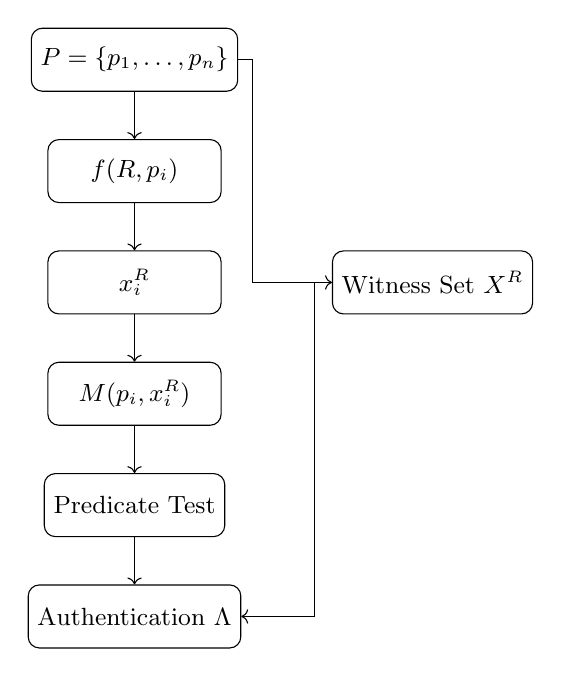
\begin{tikzpicture}[
    node distance=0.6cm, auto,
    every node/.style={
        draw, rectangle, rounded corners, align=center,
        minimum width=2.2cm, minimum height=0.8cm,
        font=\small
    }
]
    \node (P) {\(P = \{p_1,\dots,p_n\}\)};
    \node (f) [below=of P] {\(f(R, p_i)\)};
    \node (x) [below=of f] {\(x_i^R\)};
    \node (M) [below=of x] {\(M(p_i, x_i^R)\)};
    \node (Pred) [below=of M] {Predicate Test};
    \node (Auth) [below=of Pred] {Authentication \(\Lambda\)};
    \node (Xset) [right=of x, xshift=0.8cm] {Witness Set \(X^R\)};
    \draw[->] (P) -- (f);
    \draw[->] (f) -- (x);
    \draw[->] (x) -- (M);
    \draw[->] (M) -- (Pred);
    \draw[->] (Pred) -- (Auth);
    \draw[->] (P) -- ++(1.5,0) |- (Xset);
    \draw[->] (Xset) -- ++(-1.5,0) |- (Auth);
\end{tikzpicture}
\caption{Framework Overview: Mapping and Predicate Verification}
\label{fig:framework-overview}
\end{figure}

\section{Test Case: Mapping \& Union Verification}
Consider the example:
\[
P = \{3, 5, 7\}, \quad N = 2, \quad \mathcal{X} = \{0,1,\dots,9\}.
\]
Define:
\[
f(R,p) = (R \cdot p) \mod 10,\quad M(p,x) = (p + x) \mod 10.
\]

\subsection{Round 1 Calculations}
\begin{itemize}[leftmargin=0.5cm]
    \item \(x_1^1 = (1\cdot3) \mod 10 = 3\) \(\Rightarrow\) \(M(3,3) = 6\) (even)
    \item \(x_2^1 = (1\cdot5) \mod 10 = 5\) \(\Rightarrow\) \(M(5,5) = 0\) (even)
    \item \(x_3^1 = (1\cdot7) \mod 10 = 7\) \(\Rightarrow\) \(M(7,7) = 4\) (even)
\end{itemize}

\subsection{Round 2 Calculations and Explanation}
\begin{align*}
    x_1^2 &= (2 \cdot 3) \mod 10 = 6, \quad &M(3,6) &= (3+6) \mod 10 = 9  \\
    x_2^2 &= (2 \cdot 5) \mod 10 = 0, \quad &M(5,0) &= (5+0) \mod 10 = 5  \\
    x_3^2 &= (2 \cdot 7) \mod 10 = 4, \quad &M(7,4) &= (7+4) \mod 10 = 1
\end{align*}

The outputs in Round 2 are odd, so the sample predicate fails—indicating a need to adjust \(f\) or the predicate for valid authentication. The union of witness sets is:
\[
X^1 = \{3,5,7\},\quad X^2 = \{6,0,4\} \quad \Longrightarrow \quad U = \{0,3,4,5,6,7\}.
\]
A complete test requires \(U = \mathcal{X}\), ensuring full domain coverage.

\subsection{Mapping \& Union Flow Diagram}
\begin{figure}[!htbp]
\centering
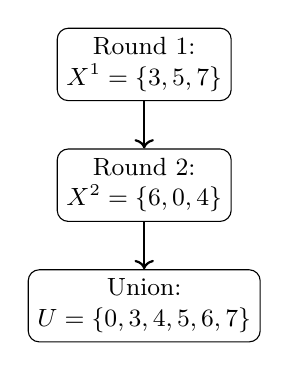
\begin{tikzpicture}[
    node distance=0.6cm, auto,
    every node/.style={
        draw, rectangle, rounded corners, align=center,
        minimum width=2cm, minimum height=0.8cm,
        font=\small
    }
]
    \node (R1) {Round 1:\\ \(X^1=\{3,5,7\}\)};
    \node (R2) [below=of R1] {Round 2:\\ \(X^2=\{6,0,4\}\)};
    \node (Union) [below=of R2] {Union:\\ \(U=\{0,3,4,5,6,7\}\)};
    \draw[->, thick] (R1) -- (R2);
    \draw[->, thick] (R2) -- (Union);
\end{tikzpicture}
\caption{Mapping \& Union Flow Across Two Rounds}
\label{fig:mapping-union}
\end{figure}

\section{Time-Dependent Key Generation}
The session key is defined as:
\[
K(t,S,r)=T(t) \oplus E\big(\lambda(t),S,r\big),
\]
where:
\begin{itemize}[leftmargin=0.5cm]
    \item \(T(t)\) is a time-derived component.
    \item \(\lambda(t)\) is a quantum-derived entropy value.
    \item \(S\) is the user secret.
    \item \(r\) is a random salt.
\end{itemize}

The function \(E(\lambda(t),S,r)\) encrypts the combination of the quantum entropy, the user secret, and the salt. The XOR operation \(\oplus\) then yields a session key with collision resistance:
\[
\Pr\Big[K(t,S,r)=K(t',S,r)\Big] \le 2^{-455} \quad \text{for } t \neq t'.
\]

\subsection{Key Generation Diagram}
\begin{figure}[!htbp]
\centering
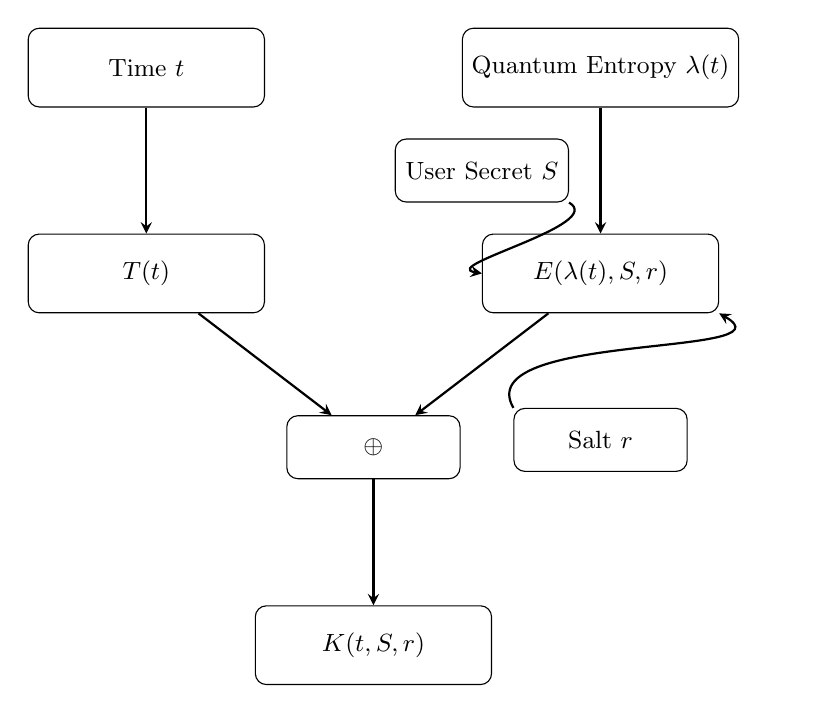
\begin{tikzpicture}[
    node distance=1.6cm and 2.2cm,
    auto,
    largebox/.style={
        draw, rectangle, rounded corners, align=center,
        font=\small, minimum width=3cm, minimum height=1cm
    },
    smallbox/.style={
        draw, rectangle, rounded corners, align=center,
        font=\small, minimum width=2.2cm, minimum height=0.8cm
    },
    line/.style={draw, -stealth, thick}
]
    \node[largebox] (Time) {Time \(t\)};
    \node[largebox, right=2.5cm of Time] (Lambda) {Quantum Entropy \(\lambda(t)\)};
    \node[largebox, below=1.6cm of Time] (T) {\(T(t)\)};
    \node[largebox, below=1.6cm of Lambda] (E) {\(E(\lambda(t), S, r)\)};
    \node[smallbox, left=0.4cm of $(Lambda)!0.5!(E)$] (Secret) {User Secret \(S\)};
    \node[smallbox, right=0.4cm of $(Lambda)!0.5!(E)$, below=1.2cm of E] (Salt) {Salt \(r\)};
    \node[smallbox, below=1.8cm of $(T)!0.5!(E)$] (XOR) {\(\oplus\)};
    \node[largebox, below=1.6cm of XOR] (K) {\(K(t, S, r)\)};

    \draw[line] (Time) -- (T);
    \draw[line] (Lambda) -- (E);
    \draw[line] (Secret.south east) to[out=-30, in=170] (E.west);
    \draw[line] (Salt.north west) to[out=120, in=-30] (E.south east);
    \draw[line] (T) -- (XOR);
    \draw[line] (E) -- (XOR);
    \draw[line] (XOR) -- (K);
\end{tikzpicture}
\caption{3.1 Time-Dependent Key Generation Diagram}
\label{fig:key-generation}
\end{figure}

% ------------ Switch to One-Column Mode for Remaining Sections ------------
\onecolumn

\section{Glossary and Assumptions}
\begin{description}[leftmargin=0.5cm, labelindent=0.5cm]
    \item[\(P\)] Set of secure primes (e.g., 256 bits) ensuring high cryptographic strength.
    \item[\(f(R,p)\)] One-way witness generation function.
    \item[\(x_i^R\)] Witness value for prime \(p_i\) at round \(R\).
    \item[\(M(p,x)\)] Homomorphic mapping function for zero-knowledge proof.
    \item[\(\mathcal{X}\)] Complete domain of witness values.
    \item[\(\Lambda\)] Overall authentication predicate.
    \item[\(T(t)\)] Time-derived component in key generation.
    \item[\(\lambda(t)\)] Quantum-derived entropy value.
    \item[\(S\)] User secret (private key).
    \item[\(r\)] Random salt value.
    \item[\(K(t,S,r)\)] Collision-resistant session key.
    \item[\(E(\lambda(t),S,r)\)] Encryption function combining quantum entropy, secret, and salt.
    \item[\textbf{Assumptions:}]
        \begin{itemize}[leftmargin=0.5cm]
            \item \(P\) consists of large, unpredictable primes.
            \item The function \(f\) is one-way and preserves secrecy.
            \item \(M\) and the union condition ensure complete domain coverage without leakage.
            \item The key generation process ensures negligible collision probability (\(2^{-455}\)).
            \item The system leverages high entropy and advanced mathematical constructs to thwart quantum and AI attacks.
        \end{itemize}
\end{description}

\section{Conclusion and Demo Integration}
To verify the Sentient Proof Framework, a reviewer should:
\begin{itemize}[leftmargin=0.5cm]
    \item Compute the mappings \(M(p,f(R,p))\) and check the predicate across rounds.
    \item Validate that the union of witness sets meets the condition \(\bigcup_{R=1}^{N} X^R = \mathcal{X}\).
    \item Test the collision resistance of the session key \(K(t,S,r)\) using multiple time samples.
\end{itemize}

\subsection{Integration with Code and Pseudocode}
A sample pseudocode for testing the protocol is:
\begin{lstlisting}
# Pseudocode for verifying the Sentient Proof Framework
for each round R:
    for each prime p in P:
        x = f(R, p)
        if Predicate(M(p, x)) is False:
            report "Authentication failed in round R for prime p"
            exit
    add all x values to witness_set_R

if union(witness_set_R for all R) != full_domain:
    report "Union condition not met"
else:
    report "Mapping and union conditions satisfied"

# Key generation test:
for different times t1, t2:
    key1 = T(t1) XOR E(lambda(t1), S, r)
    key2 = T(t2) XOR E(lambda(t2), S, r)
    if key1 == key2:
        report "Collision detected"
    else:
        report "Unique keys generated"
\end{lstlisting}

\subsection{Demo Output}
Below is the example output from the Python protocol demonstration:
\begin{lstlisting}
Enter seed phrase: [Tzq7431GYua711X236894B6117065704FFFrw7739]
Use flexible password requirements? (y/n): YES
    ENTER Basic password required (minimum 8 characters)
    Enter password (min 8 chars): LOVE1234
Use custom salt? (y/n): YES
Enter custom salt: [627683761gjhsvjdv]
Generated salt: 538283e9eef56222e00defd6e57a0ed4
Use custom color mapping? (y/n): YES

=== Custom Color-Direction Mapping Setup ===
Choose direction for Yellow: `up`
Choose direction for Green: `down`
Choose direction for Blue: `left`
Choose direction for Red: `right`

Running protocol...
2025-03-20 16:39:54,835 [INFO] Session: Protocol started
Using seed: som...234
Security level: 10
2025-03-20 16:39:54,836 [INFO] Session: Generated 12 entropy layers
Initializing Mentri verifier, Challenge Protocol Simulation for SIGMA Protocol verification with password length `8`
2025-03-20 16:39:54,837 [INFO] Session: Sentient protocol initialized, starting interactive verification

=== Sentient Verification (8 Rounds) ===

--- Round 1 ---
Character shown in these color-coded hyperplanes:
Hyperplane 0 (Yellow): X!5TWU6ZYV
Hyperplane 1 (Green): @9FCAE7B8D
Hyperplane 2 (Blue): 10KIHMLGJ$
Hyperplane 3 (Red): Q3S4PRO2&N
Enter direction for this character: left

--- Round 2 ---
Character shown in these color-coded hyperplanes:
Hyperplane 0 (Yellow): @9D8C$AZBY
Hyperplane 1 (Green): G01IJKEH2F
Hyperplane 2 (Blue): MOP3&Q!N4L
Hyperplane 3 (Red): 6V5URW7XTS
Enter direction for this character: left

--- Round 3 ---
Character shown in these color-coded hyperplanes:
Hyperplane 0 (Yellow): MN&K0JLO12
Hyperplane 1 (Green): TUSPRV!34Q
Hyperplane 2 (Blue): @7XY65BZWA
Hyperplane 3 (Red): FHGD89I$EC
Enter direction for this character: down

--- Round 4 ---
Character shown in these color-coded hyperplanes:
Hyperplane 0 (Yellow): !FCBDGE45A
Hyperplane 1 (Green): &7MIHJK68L
Hyperplane 2 (Blue): O9TQP$0NRS
Hyperplane 3 (Red): 3Y@XZVU21W
Enter direction for this character: up

--- Round 5 ---
Character shown in these color-coded hyperplanes:
Hyperplane 0 (Yellow): 1AGEFBC2D3
Hyperplane 1 (Green): M!54&LIKJH
Hyperplane 2 (Blue): R8QP7T6OSN
Hyperplane 3 (Red): @YU0ZW$9XV
Enter direction for this character: up

--- Round 6 ---
Character shown in these color-coded hyperplanes:
Hyperplane 0 (Yellow): !PQR5&6NSO
Hyperplane 1 (Green): WTU9ZY87XV
Hyperplane 2 (Blue): CD0BF1AE@$
Hyperplane 3 (Red): J43HI2GMKL
Enter direction for this character: right

--- Round 7 ---
Character shown in these color-coded hyperplanes:
Hyperplane 0 (Yellow): 7POSQN6R&5
Hyperplane 1 (Green): XTYUW8ZV9$
Hyperplane 2 (Blue): @0FDA2EC1B
Hyperplane 3 (Red): 4KGJHLM3I!
Enter direction for this character: right

--- Round 8 ---
Character shown in these color-coded hyperplanes:
Hyperplane 0 (Yellow): PRO$TN8S9Q
Hyperplane 1 (Green): Z0VUX21W@Y
Hyperplane 2 (Blue): EC!3GABDF4
Hyperplane 3 (Red): &6JMHL57KI
Enter direction for this character: left

...
--- Auth Complete, Enter Proof Authentication Validation over Holomorphic Witness Accumulation Protocol ---
2025-03-20 16:40:26,413 [INFO] Session: 
Sentient verification completed with 8 rounds for witness accumulation responses from prover framework!
2025-03-20 16:40:26,413 [INFO] Session: Sentient verification successful.
2025-03-20 16:40:26,420 [INFO] Authenticated puzzle proof confirmed. Initiating prime search: 10 primes, 256 bits each.
--- Prime Discovery ---
2025-03-20 18:15:23,456 [INFO] Starting prime search for 10 primes of 256 bits...
2025-03-20 18:15:23,506 [INFO] Prime found: 72535155591949439583286653989606050638591796748057459243898442446889359734351 (attempt 32001, space 1, orbital 0)
2025-03-20 18:15:23,556 [INFO] Prime found: 114659080029911085649738125081131359318367453877474201025890203571729232791779 (attempt 7001, space 2, orbital 0)
2025-03-20 18:15:23,606 [INFO] Prime found: 91577035533705166901727191452814850436997785142259167060035943042411784618011 (attempt 7002, space 2, orbital 0)
2025-03-20 18:15:23,656 [INFO] Prime found: 110009007663200311160512944794414545006693555307539513337757101166564763025363 (attempt 1, space 3, orbital 0)
2025-03-20 18:15:23,706 [INFO] Prime found: 65518156838111088812608323364659122860705942230670359420440566338719175678611 (attempt 5001, space 3, orbital 0)
2025-03-20 18:15:23,756 [INFO] Prime found: 108276446240531873906224314193260889515000949244847682295553719904298102498283 (attempt 11001, space 3, orbital 0)
2025-03-20 18:15:23,806 [INFO] Prime found: 77255897119620173404004970075130021593636522924889396867097673772946645262731 (attempt 21001, space 3, orbital 0)
2025-03-20 18:15:23,856 [INFO] Prime found: 93518768839367699306618891215015923010236697995570791221358916024856928641679 (attempt 1001, space 4, orbital 0)
2025-03-20 18:15:23,906 [INFO] Prime found: 89462869922531802743259698491193138346675469976131320885085755262732213889231 (attempt 10001, space 4, orbital 0)
2025-03-20 18:15:23,956 [INFO] Prime found: 70815420785542809142914917207083411357054177783550586228725029172891825716079 (attempt 16001, space 4, orbital 0)
--- Summary ---
2025-03-20 18:15:23,956 [INFO] Orbital rotation 0: 10 primes found in 2.50s
2025-03-20 18:15:23,956 [INFO] Total primes found: 10 in 2.50s across 10 spaces and 4 orbital rotations
2025-03-20 18:15:23,956 [INFO] Selected top 10 largest primes
--- Session Results ---
2025-03-20 18:15:23,956 [INFO] Session: Generated 10 holy primes
Proofs Generated:
2025-03-20 18:15:23,957 [INFO] Proof generated for prime 72535155591949439583286653989606050638591796748057459243898442446889359734351
2025-03-20 18:15:23,958 [INFO] Proof generated for prime 114659080029911085649738125081131359318367453877474201025890203571729232791779
2025-03-20 18:15:23,959 [INFO] Proof generated for prime 91577035533705166901727191452814850436997785142259167060035943042411784618011
2025-03-20 18:15:23,960 [INFO] Proof generated for prime 110009007663200311160512944794414545006693555307539513337757101166564763025363
2025-03-20 18:15:23,961 [INFO] Proof generated for prime 65518156838111088812608323364659122860705942230670359420440566338719175678611
2025-03-20 18:15:23,962 [INFO] Proof generated for prime 108276446240531873906224314193260889515000949244847682295553719904298102498283
2025-03-20 18:15:23,963 [INFO] Proof generated for prime 77255897119620173404004970075130021593636522924889396867097673772946645262731
2025-03-20 18:15:23,964 [INFO] Proof generated for prime 93518768839367699306618891215015923010236697995570791221358916024856928641679
2025-03-20 18:15:23,965 [INFO] Proof generated for prime 89462869922531802743259698491193138346675469976131320885085755262732213889231
2025-03-20 18:15:23,966 [INFO] Proof generated for prime 70815420785542809142914917207083411357054177783550586228725029172891825716079
2025-03-20 18:15:23,966 [INFO] Session: Generated ECDSA signature
2025-03-20 18:15:23,966 [INFO] Session: Protocol completed successfully
\end{lstlisting}
\textbf{END OF DEMO OUTPUT}

We rely on dense entropy hashing and lattice-based geometric hashing to generate effective entropy, with a very efficient prime search algorithm that can generate large prime numbers instantly with an absolute value equal to prime.

\begin{center}
\textbf{Contact:}\\
Dylan Kawalec, \href{mailto:dylan@coin.fi}{dylan@coin.fi} \quad\quad
Arvin Bhangu, \href{mailto:arvin@coin.fi}{arvin@coin.fi}\\[1ex]
\textbf{Organization:} Coin.fi Research Team
\end{center}

\section*{References}
\begin{enumerate}
\item \href{https://eni6ma.gitbook.io}{eni6ma.gitbook.io} - Additional documentation and resources.
\end{enumerate}

\end{document}

